\documentclass[a4paper,12pt]{article}
\usepackage[utf8]{inputenc}
\usepackage{xcolor}
\usepackage{url}
\usepackage[T2A]{fontenc}
\usepackage{graphicx}
\usepackage[margin=80pt]{geometry}

\usepackage[english,serbian]{babel}

\begin{document}

\title{\textbf{Zene u programiranju\\} \small{Seminarski rad u okviru kursa\\Tehnisko i naucno pisanje\\ Matematicko fakultet}}

\author{Jelena Velickovic\\ mi21203@alas.matf.bg.ac.rs \and Bojana Zagorac\\ mi22135@alas.matf.bg.ac.rs \and Milos Bigovic\\ mi22149@alas.matf.bg.ac.rs \and Zorana Jevtic\\ mi22148@alas.matf.bg.ac.rs}

\date{\textit{\center{Novembar, 2022.}}}

\maketitle

\begin{abstract}
    U ovom tekstu je ukratko objasnjen doprinos zena u programiranju uz priloge. Takodje, bice reci o
    brojnosti zena koje se time bave, kao i o Adi Bajron, najistaknutijom zenom programerom. Sustina 
    ovog teksta je razbijanje predrasude da se programiranjem bave iskljucivo muskarci, odnosno da je 
    programiranje "muski posao". 
\end{abstract}


\color{blue}\tableofcontents

\newpage
\color{black}\section{Uvod}

\newpage
\section{Ada Bajron}

\begin{flushleft}
    Ejda Bajron(1815-1852.), poznata kao Ada, smatra se prvim programerom zbog svog programa kojim se pomocu analiticke masine izracunavaju Bernulijevi brojevi. Odnosno, ucestvovala je u realizaciji projekta analiticke masine funansijski i svojim idejama. Njena najznacajnija ideja u realizaciji tog projekta je bio prenos kontrole i rad sa ciklusima. Iako se primarno bavila matematikom, to nije znacilo da se tu zaustavljaju njena interesovanja. Za razliku od mnogih u to doba, bila je inovativna smatrajuci da se analiticka masina moze upotrebljavati za opstije stvari, kao i u naucne svrhe. To je u buducnosti i realizovano, dakle savremeni racunari se upravo uklapaju u tu njenu zamisao.Upoznavsi poznatog matematicara Carlsa Bebidza, nakon nekog vremena mu se pridruzila u projektu kao njegov tumac. To jest, jasno je opisala kako ce masina funkcionisati, cime je doprinela računarskoj nauci. Objasnila je da je sustina rada analiticke masine tkanje algebarskih obrazaca poput Zakardove masine koja je radila po principu kreiranja slika na osnovu busenih kartica. Predmet svojih proucavanja i rada je nazivala naukom i operacijama, medjutim to je zapravo racunarstvo. Nije ni cudno to sto je razmisljala na tako genijalan nacin, s obzirom na to da je spojila mastovitost sa racionalnoscu. Umetnicku crtu je nasledila od oca lorda Bajrona, romanticarskog pesnika, dok je zahvaljujuci majcinom uticaju uspela da stvori ravnotezu i izbegne povrsan pristup. Bez obzira na to sto su neki naucnici pokusavali da ospore njen rad i doprinos, mnogi su odbacivali ovo tumacenje. Razlog osporavanja je bio cuvanje moci u rukama muskarca kao i predrasude prema zenama koje se bave programiranjem zbog spoznaje vaznosti i znacaja te naucne oblasti. Vrhunac njene karijere je programski jezik nazvan Ada u njenu cast, kao i priznanje koje dobija svake godine 15. oktobra, pocevsi od 2009. godine kako bi se istakao naucni rad i doprinos zena koji je zanemaren i nipodastavan. Na slici 1, prikazana je Ada Bajron.
\end{flushleft}

\begin{figure}
    \centering
    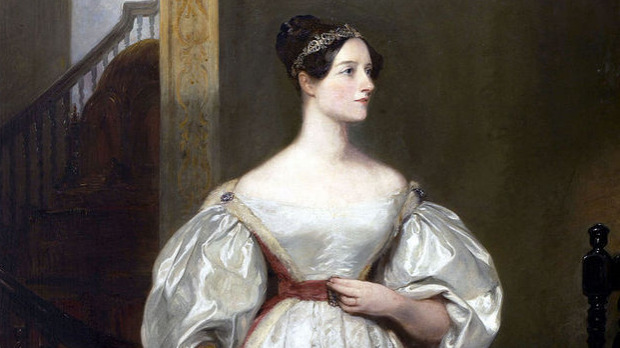
\includegraphics[width = .6\textwidth]{figs/adabajron.jpg}
    \caption{Ада Бајрон}
    \label{fig:my_label}
\end{figure}


\end{document}
